\subsection{Logarithms and Their Applications}
$$b^{x} = y \leftrightarrow x = log_{b}y$$
$$b^{log_{b}y} = y$$

\subsubsection{Logarithms and Binary Search}

\begin{figure}[H]
  \centering
     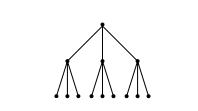
\includegraphics[scale=0.9]{./2_7.png}
  \label{fig:demo-diagram2-4}
  \caption{ A height \emph{h} tree with \emph{d} children per node as \emph{$d^{h}$} leaves. Here $h=2$ and $d=3$}
\end{figure}


\subsubsection{Logarithms Trees}

\subsubsection{Logarithms and Bits}

\subsubsection{Logarithms and Multiplication}

\begin{align*}
	&log_{a}(xy) = log_{a}(x) + log_a(y) \\
	&log_{a} n^{b} = b \cdot log_{a} n \\
	&a^{b} = e^{(ln(a^{b}))} = e^{(b(ln(a)))}
\end{align*}

\subsubsection{Fast Exponentiation}

\subsubsection{Logarithms and Summations}

\emph{Harmonic Numbers}: 
$$H(n) = \sum_{i=1}^{n} \frac{1}{i} \sim ln(n)$$

\subsubsection{Logarithms and Criminal Justice}


\begin{figure}[H]
  \centering
     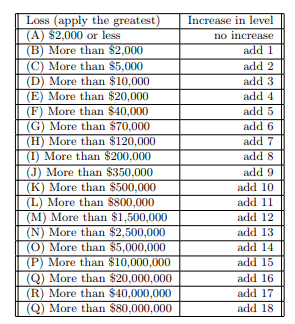
\includegraphics[scale=0.9]{./2_8.png}
  \label{fig:demo-diagram2-8}
  \caption{The Federal Sentencing Guidelines for fraud}
\end{figure}

\noindent\fbox{\parbox{\textwidth}{%
\emph{Take-Home Lesson: } Logarithms arise whenever things are repeatedly halved or doubled
}%
}
